\documentclass[10pt,a4paper]{article}
\usepackage[utf8]{inputenc}
\usepackage{amsmath}
\usepackage{amsfonts}
\usepackage{makeidx}
\usepackage{draftwatermark}
\SetWatermarkText{CONFIDENTIAL}
\SetWatermarkColor[gray]{0.5}
\SetWatermarkScale{4}
\usepackage{listings}
\usepackage{color}

\definecolor{mygreen}{rgb}{0,0.6,0}
\definecolor{mygray}{rgb}{0.5,0.5,0.5}
\definecolor{mymauve}{rgb}{0.58,0,0.82}

\lstset{ %
  backgroundcolor=\color{white},   % choose the background color; you must add \usepackage{color} or \usepackage{xcolor}
  basicstyle=\footnotesize,        % the size of the fonts that are used for the code
  breakatwhitespace=false,         % sets if automatic breaks should only happen at whitespace
  breaklines=true,                 % sets automatic line breaking
  captionpos=b,                    % sets the caption-position to bottom
  commentstyle=\color{mygreen},    % comment style
  deletekeywords={...},            % if you want to delete keywords from the given language
  escapeinside={\%*}{*)},          % if you want to add LaTeX within your code
  extendedchars=true,              % lets you use non-ASCII characters; for 8-bits encodings only, does not work with UTF-8
  frame=single,                    % adds a frame around the code
  keepspaces=true,                 % keeps spaces in text, useful for keeping indentation of code (possibly needs columns=flexible)
  keywordstyle=\color{blue},       % keyword style
  language=Octave,                 % the language of the code
  morekeywords={*,...},            % if you want to add more keywords to the set
  numbers=left,                    % where to put the line-numbers; possible values are (none, left, right)
  numbersep=5pt,                   % how far the line-numbers are from the code
  numberstyle=\tiny\color{mygray}, % the style that is used for the line-numbers
  rulecolor=\color{black},         % if not set, the frame-color may be changed on line-breaks within not-black text (e.g. comments (green here))
  showspaces=false,                % show spaces everywhere adding particular underscores; it overrides 'showstringspaces'
  showstringspaces=false,          % underline spaces within strings only
  showtabs=false,                  % show tabs within strings adding particular underscores
  stepnumber=2,                    % the step between two line-numbers. If it's 1, each line will be numbered
  stringstyle=\color{mymauve},     % string literal style
  tabsize=2,                       % sets default tabsize to 2 spaces
  title=\lstname                   % show the filename of files included with \lstinputlisting; also try caption instead of title
}
\usepackage{amssymb}
\usepackage{graphicx}
\usepackage{float}
\usepackage{hyperref}
%\usepackage[Sonny]{fncychap}
\floatstyle{boxed}
\restylefloat{figure}
\usepackage[left=2cm,right=2cm,top=2cm,bottom=2cm]{geometry}
\newcommand{\HRule}{\rule{\linewidth}{0.5mm}}
\begin{document}
\begin{titlepage}
\begin{center}

% Upper part of the page. The '~' is needed because \\
% only works if a paragraph has started.
%
\includegraphics[width=0.15\textwidth]{./logo}~\\[1cm]

%\textsc{\LARGE University of Beer}\\[1.5cm]

\textsc{\Large Project Proposal}\\[0.5cm]

% Title
\HRule \\[0.4cm]
{ \huge \bfseries Project Quad \\[0.4cm] }

\HRule \\[1.5cm]

% Author and supervisor
\begin{minipage}{0.4\textwidth}
\begin{flushleft} \large
\emph{Author:}\\
Andy \textsc{Fang}
\end{flushleft}
\end{minipage}
\begin{minipage}{0.4\textwidth}
\begin{flushright} \large
\emph{Supervisor:} \\
Dr.~Mark \textsc{Brown}
\end{flushright}
\end{minipage}

\vfill

% Bottom of the page
{\large \today}

\end{center}
\end{titlepage}
%\maketitle
\newpage
\tableofcontents 
\newpage
\section{Basic Concept}
\subsection{Quadcopter}
\subsubsection{Defination}
A quadcopter, also called a quadrotor helicopter, quadrocopter, quadrotor, is a multicopter that is lifted and propelled by four rotors.\cite{cite1}
\begin{figure}[h!]
  
  \centering
    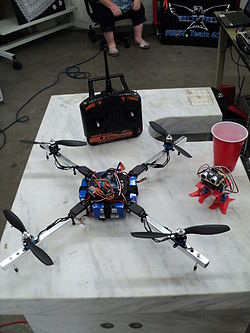
\includegraphics[width=0.3\textwidth]{./Pictures/250px-ReuseumMakerFaireQuadrotor.JPG}
    \caption{A Maker Faire quadcopter in Garden City, Idaho\cite{cite1}}\\
\end{figure}
\subsubsection{Flight Control}
\begin{figure}[h!]
  
  \centering
    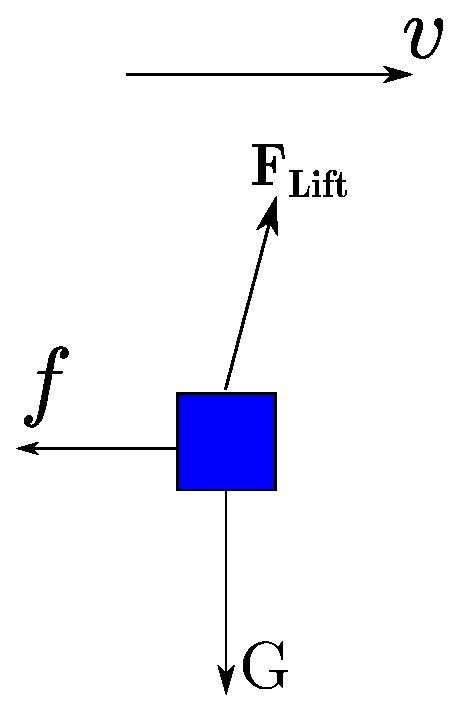
\includegraphics[width=0.3\textwidth]{./Pictures/flying.eps}
    \caption{The forces effected on the quadcopter while making stable movement.}\\
\end{figure}
%\newpage
\textbf{[ Hover ]}
\begin{figure}[H]
  
  \centering
    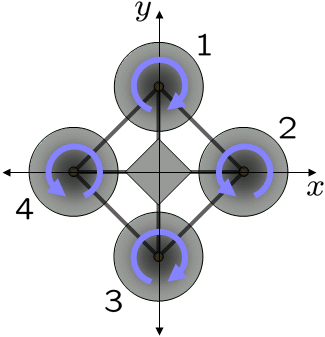
\includegraphics[width=0.3\textwidth]{./Pictures/Quadrotor_yaw_torque.png}
    \caption{The example model of quadcopter.}\\
\end{figure}


Each rotor porduces both thrust and torque. If all the rotors are spining at the same angular velocity, and as the example shows, with rotor 1,3 spining clockwise and rotor 2,4 spining counterclockwise, the angular acceleration on the yaw-axis will be zero. 
This is the method to hovering.

\textbf{[ Yaw ]}\\
\begin{figure}[H]
  
  \centering
    
\includegraphics[width=0.3\textwidth]{./Pictures/yaw.png}
    \caption{Yaw control}
\end{figure}
The method of making yaw control can be done by adjusting the angular velocity of one pair of rotors.\\
\textbf{[ Pitch ]}\\
\begin{figure}[H]
  
  \centering
    
\includegraphics[width=0.3\textwidth]{./Pictures/pitch.png}
    \caption{Pitch control}
\end{figure}
The method of making pitch control can be done by increasing one rotor's spinning velocity and decreasing the opposite rotor's spinning velocity.\\
\textbf{[ Roll ]}\\
\begin{figure}[H]
  
  \centering
    
\includegraphics[width=0.3\textwidth, angle=90]{./Pictures/pitch.png}
    \caption{Roll control}
\end{figure}
The method of making roll control is similar to making pitch control.\\
It can be done by increasing one rotor's spinning velocity and decreasing the opposite rotor's spinning velocity.\\

\textbf{The eeeeeeeeeeasy way}\\
Use the ardupilot\cite{cite2} library.\\
\textbf{The harrrrrrrrrrd way}\\
Write the control system complete from scratch.\\
Which is possible, but might take a loooooooooong time.
\newpage

\begin{thebibliography}{9}

\bibitem{cite1}
  Wikipedia ,
  \emph{Quadcopter}.
  \url{https://en.wikipedia.org/wiki/Quadcopter}
\bibitem{cite2}
  GitHub ,
  \emph{ardupilot}.
  \url{https://github.com/diydrones/ardupilot},\url{http://ardupilot.com/}

\end{thebibliography}



\end{document}